\documentclass[14pt, fleqn, xcolor={dvipsnames, table}]{beamer}
\usepackage[T2A]{fontenc}
\usepackage[utf8]{inputenc}
\usepackage[english,russian]{babel}
\usepackage{amssymb,amsfonts,amsmath,mathtext}
\usepackage{cite,enumerate,float,indentfirst}
\usepackage{cancel}

\usepackage{tikz}                   
\usetikzlibrary{shadows}

% \usepackage{enumitem}
% \setitemize{label=\usebeamerfont*{itemize item}%
%   \usebeamercolor[fg]{itemize item}
%   \usebeamertemplate{itemize item}}

\graphicspath{{images/}}

\usetheme{Madrid}
\usecolortheme{seahorse}
\renewcommand{\CancelColor}{\color{red}}

\setbeamercolor{footline}{fg=Blue!50}
\setbeamertemplate{footline}{
  \leavevmode%
  \hbox{%
  \begin{beamercolorbox}[wd=.333333\paperwidth,ht=2.25ex,dp=1ex,center]{}%
    И. Кураленок, Н. Поваров, Яндекс
  \end{beamercolorbox}%
  \begin{beamercolorbox}[wd=.333333\paperwidth,ht=2.25ex,dp=1ex,center]{}%
    Санкт-Петербург, 2015
  \end{beamercolorbox}%
  \begin{beamercolorbox}[wd=.333333\paperwidth,ht=2.25ex,dp=1ex,right]{}%
  Стр. \insertframenumber{} из \inserttotalframenumber \hspace*{2ex}
  \end{beamercolorbox}}%
  \vskip0pt%
}
\newcommand\indentdisplays[1]{%
     \everydisplay{\addtolength\displayindent{#1}%
     \addtolength\displaywidth{-#1}}}
\newcommand{\itemi}{\item[\checkmark]}

\AtBeginSection[]
{  
 \addtocounter{framenumber}{-1}
 \begin{frame}<beamer>
   \frametitle{План}
   \small
   \tableofcontents[currentsection]
 \end{frame}
}

\title{Линейные модели: жатые чувства, SVM (начнем)\\\small{}}
\author[]{\small{%
И.~Куралёнок,
Н.~Поваров}}
\date{}

\begin{document}

\begin{frame}

\maketitle
\small
\begin{center}
\vspace{-60pt}
\normalsize {\color{red}Я}ндекс \\
\vspace{80pt}
\footnotesize СПб, 2015
\end{center}
\end{frame}

\section{Постановка задачи восстановления сигнала}
\subsection{Пример}
\begin{frame}{Пример}
Сергей Юрьевич любит смотреть телевизор и рассуждать. Есть мнение, что в основном по телевизору "льют воду".
Надо понять как часто надо обращать внимание на то, что проиходит на экране, чтобы не упустить "нить".
\end{frame}
\begin{frame}{Пример: постановка задачи}
\begin{center}
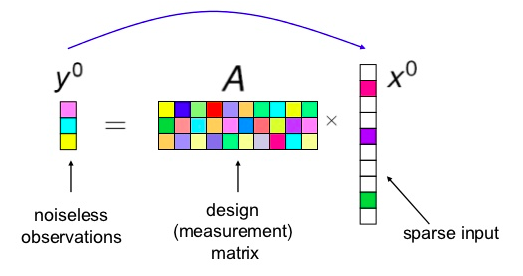
\includegraphics[width=0.6\textwidth]{CS-ProblemSetup-1.png}
\end{center}
\vspace{-2em}
\small
\begin{itemize}
  \item В телевизоре хотят сказать $x^0$ ($\beta^*$)
  \item Говорят много ($n$), но информации там мало ($k$)
  \item Матрица $A$ ($X$) --- язык передачи
  \item $y^0$ ($y$) --- то, что мы видим
\end{itemize}
\footnotesize
$\Rightarrow$ Хотим устроить язык передачи так, чтобы минимизировать количество наблюдений, для восстановления $\hat{\beta}$ как можно ближе к правде $\beta^*$\\
\tiny Картинка из Tutorial ICML2010 by Irina Rish \& Genady Grabarnik
\end{frame}

\begin{frame}{Restricted isometry property}
Пусть $A$ --- матрица $m\times n$, $1 \le s \le n$. Если существует $\delta_s$, такая что:
$$
(1-\delta_s)\|y\|^2_2 \le \|A_sy\|^2_2 \le (1+\delta_s)\|y\|^2_2
$$
для любой подматрицы $A_s$, состоящей из $s$ столбцов матрицы $A$, и $\forall y$. Тогда матрица $A$ удовлетворяет $s$-ограниченным изометрическим свойством ($s$-Restricted Isometry Property).
\end{frame}

\begin{frame}{Решение точной задачи}
\begin{center}
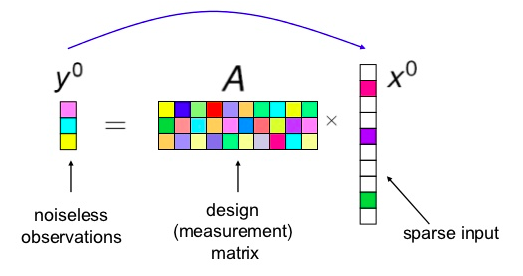
\includegraphics[width=0.6\textwidth]{CS-ProblemSetup-1.png}
\end{center}
\vspace{-1em}

\small
Если язык (матрица $A$) устроен ``правильно'' (удовлетворяет k-RIP), то решение:
$$
\min_{x : y^0 = A x} \|x\|_1 
$$
восстановит загаданный $x^0$. Или в наших обозначениях:
$$
\beta^* = \min_{\beta : y = X \beta} \|\beta\|_1
$$
\end{frame}

\begin{frame}{Сюрприз compressed sensing}
\small
$$
y = X\beta + \epsilon
$$
Если компоненты матрицы $X$ независимые, одинаково распределенные, нормальные, то $\beta$ можно восстановить точно с большой вероятностью:
\begin{itemize}
  \item из $O(k log(\frac{n}{k}))$ измерений;
  \item решив оптимизацию
    $$\begin{array}{l}
    \arg \min_\beta\|\beta\|_1\\
    \|y - X\beta\| < \epsilon
    \end{array}$$
\end{itemize}
$\Rightarrow$ где-то мы уже такое видели
\end{frame}

\begin{frame}{Линейная регрессия vs. восстановление сигнала}
\begin{itemize}
  \item Решают одну и ту же задачу
  \item Одни и те же алгоритмы
  \item Учиться сложнее:
  \begin{itemize}
    \item нету влияния на построение матрицы $X$;
    \item в частности нет гарантий на свойства матрицы $X$;
    \item наличие в $\beta$ большого количество нулей -- лишь наше предположение.
  \end{itemize}
\end{itemize}
\end{frame}

\subsection{Разложение сигнала в Фурье и постановка в нахождении коэффициентов}
\begin{frame}{Постановка в терминах RFP I}
\small
Будем рассматривать множество возможных наблюдений как ось времени, тогда можно рассматривать передачу информации о загаданном $\beta^*$ как моделирование сигнала через разложение в Фурье. При этом, для простоты, будем считать, что количество возможных наблюдений совпадает с размерностью вектора $\beta^*$, в этом случае мы можем рассматривать преобразование как линейную систему DFT: 
$$\begin{array}{rl}
z & = \mathcal{F} \beta^* \\
z_\omega& = \sum_{t = 0}^n \beta_t e^{-2\pi i \omega t \over n}
\end{array}$$
Возвращаясь к примеру, для Сергея Юрьевича, если он смотрел до конца, и все хорошо понимал, ситуация выглядит как-то так:
$$
\hat{\beta} = \mathcal{F}^{-1} \mathcal{F} \beta^* = \frac{1}{n}\mathcal{F^*} \mathcal{F} \beta^* = \beta^*
$$
\end{frame}

\section{LASSO для восстановления сигнала}

\begin{frame}{Постановка в терминах RFP II}
  $$\begin{array}{l}
  \arg \min_\beta\|\beta\|_1\\
  \|y - X\beta\| < \epsilon
  \end{array}$$
 В новых обозначениях:
$$\begin{array}{l}
\arg \min_\beta \|\beta\|_1 \\
\|(\mathcal{F}\beta)_\Omega - (\mathcal{F}\beta^*)_\Omega\| < \epsilon
\end{array}$$
где $\Omega$ --- множество моментов наблюдения.
\end{frame}

\begin{frame}{LASSO для восстановления сигнала}
Для начала решим задачу в которой наблюдения точные:
$$
z = (\mathcal{F}\beta^*)_k, k \in \Omega
$$
При этом будем решать 
$$\begin{array}{l}
\arg \min_\beta \|\beta\|_1 \\
(\mathcal{F}\beta)_k = (\mathcal{F}\beta^*)_k, k \in \Omega
\end{array}$$
с равными размерностями $\beta^*$ и $\mathcal{F}\beta^*$. Оказывается, что $\mathcal{F}^{-1} \mathcal{F}$ --- RIP. Так что $\hat{\beta} = \beta^*$.
\end{frame}

\subsection{Теорема о качестве восстановленного сигнала (Candes et al. 2006)}
\begin{frame}{Теорема о качестве восстановленного сигнала для RFP}
\small
\begin{theorem}[Candes et al. (2006)]
\begin{itemize}
\item[--] $\beta\in\mathbb{C}^n, |\{i \in \mathbb{Z}_n|\beta^*_i \ne 0\}| = S$ 
\item[--] $\Omega \subset \mathbb{Z}_n$ --- одно из равновероятных множеств фиксированного размера $|\Omega|$
\item[--] зафиксируем точность $B$
\end{itemize}
\vspace{-1em}
$\Rightarrow$ c вероятностью $P \ge 1 - O(n^{-B})$ мы можем точно восстановить $\hat{\beta} = \beta^*$, если:
$$
|\Omega| \ge C^{'}_B S \log n
$$
где $C^{'}_B \simeq 23(B + 1)$
\end{theorem}
\end{frame}

\begin{frame}{Выводы из теоремы}
\begin{itemize}
  \item Теорема рассказывает о свойствах случайной DFT проекции
  \item Загаданный вектор $\beta^*$ может быть восстановлен:
  \begin{itemize}
    \item с высокой вероятностью
    \item используя LASSO
    \item количество наблюдений пропорционально количеству ненулей в ``загаданном'' сигнале
  \end{itemize}
\end{itemize}
\end{frame}

\begin{frame}{Упрощение рандома}
В теореме $\Omega$ равномерно распределена по всем множествам фиксированного размера. Такое сложно генерировать. Значительно проще $\Omega^{'}: \forall j \in \mathbb{Z}_n, P(j \in \Omega) = \tau$. \\
$\Rightarrow$ Для таких проекций вероятность восстановить сигнал примерно такая же.
\end{frame}

\subsection{Стабильность решения: RIP, RRfND (Candes et al. 2006)}
\begin{frame}{Стабильно ли решение?}
\small
Интересны два вида ``стабильности'':
\begin{description}
  \item[стабильность:] маленькие изменения в решении при малом изменении в наблюдениях (изменения в загаданном);
  \item[робастность:] устойчивость к шуму в данных (неточно померяли отлик $y$).
\end{description}
Если мы уже решили проблему построения $T$ (множества загаданных ненулей), то решение стабильно:
$$
\hat{\beta} = (\mathcal{F}^*_{T,\Omega}\mathcal{F}_{T,\Omega})^{-1}\mathcal{F}^*_{T,\Omega}y
$$
Из доказательства теоремы о восстановлении сигнала $\mathcal{F}^*_{T,\Omega}\mathcal{F}_{T,\Omega} \succeq \delta E$ c высокой вероятностью при условии на $\Omega$. А вот с робастностью все сложнее...
\end{frame}

\begin{frame}{Можно ли как-то подругому построить $X$?}
Пока Сергей Юрьевич получал закодированный в Фурье сигнал и раскодировал его обратным Фурье. А что, если кодировани и раскодирование сигнала происходит как-то иначе. Положим, что так:
$$
\hat{\beta} = \Phi^{-1} \Phi \beta^* = \Psi \Phi \beta^*
$$
Будем рассматривать ортонормированные $\Phi, \Psi$
\end{frame}

\begin{frame}{Когерентность базисов}
\small
\begin{definition}
Для пары ортонормированных базисов назовем
$$
\mu(\Phi, \Psi) = \sqrt{n}\max_{i,j} |(\phi_i, \psi_j)|
$$
\textbf{когерентностью}.
\end{definition}
\begin{itemize}
  \item Заметим, что $1 \le \mu(\Phi,\Psi) \le \sqrt{n}$
  \item В случае Фурье получается экстремально хороший случай: $\mu(DFT,IDFT) = 1$
\end{itemize}
\end{frame}

\begin{frame}{Теорема о качестве восстановленного сигнала для произвольных базисов}
\small
\begin{theorem}[Candes and Romberg (2006)]
Для фиксированной $\delta > 0$ и $\beta^* \in \mathbb{R}^n$, $|\{i | \beta^*_i \ne 0\}| < S$. Выберем $\Omega$ точек для наблюдения равномерно из $\mathbb{Z}_n$ без повторений. Если
$$|\Omega| \ge C \mu^2(\Phi,\Psi)S\log {n\over\delta}$$
тогда решение LASSO:
$$\begin{array}{l}
\hat{\beta} = \arg \min_{\beta \in \mathbb{R}^n} \|\beta\|_1 \\
(\Phi \beta)_\Omega = (\Psi \beta^*)_\Omega
\end{array}$$
восстановит $\hat{\beta} = \beta^*$ с вероятностью $1 - \delta$
\end{theorem}
\end{frame}

\subsection{LASSO persistency theorem (Bickel et al., 2009)}
\begin{frame}{Возвращаемся к случаю шумных наблюдений}
\small
Воспользовавшись построенной теорией для точных наблюдений, введем ряд дополнительных ограничений:
\begin{enumerate}
  \item Вводим ограничение на модельную матрицу, что она $k$-RIP 
  % $$\begin{array}{l}
  % \exists \delta(S = |\{i | x \ne 0\}|): \\
  % (1-\delta(S)) \|x\|_2 \le \|Ax\|_2 \le (1 + \delta(S)) \|x\|_2
  % \end{array}$$
  \item В введенных условиях получаем ограничение на робастность в рамках восстановления сигнала
  \item Переходим от когерентности к условиям на собственные числа модельной матрицы
\end{enumerate}
\end{frame}
\begin{frame}{LASSO persistency theorem}
Во введенных условиях оказывается, что (LASSO persistency theorem, Bickel et al., 2009):
$$
\|\hat{\beta} - \beta^*\| \le O\left(\sqrt{\log n \over m}\right)
$$
Ура, мы научились измерять смещение $\hat{\beta}$ в зависимости от условий задачи. К сожалению в очень жестких условиях.
\end{frame}

\begin{frame}{Что мы узнали про CS}
\small
\begin{enumerate}
  \item Можно ставить задачу по восстановлению сигнала
  \item Для решения задачи нам понадобится рандомно выбирать точки наблюдения
  \item Оказывается, что решать подобные задачи нужно тем же самым LASSO
  \item Эффективность решения зависит от того, как построить ``язык передачи информации''
  \item Одним из самых хороших универсальных языков (c минимально возможной когерентностью) является DFT/IDFT
  \item C помощью механизма CS можно доказать устойчивость решения LASSO
\end{enumerate}
\end{frame}

\section{Support vector machines}
\subsection{Идея метода}
\begin{frame}{SVM(воспоминания о былом)}
\begin{itemize}
  \item Последний из линейных методов, который мы рассмотрим подробно.
  \item Rocket science до конца 90-х, по крайней мере в задачах классификации.
\end{itemize}
\end{frame}

\begin{frame}{SVM на пальцах}
\begin{itemize}
  \item Максимальный зазор.
  \item Нелинейные преобразования.
\end{itemize}
\begin{center}
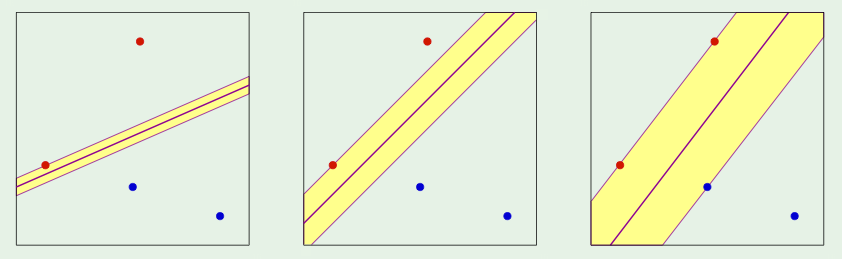
\includegraphics[width=0.9\textwidth]{SVM_1.png}
\end{center}
\end{frame}

\begin{frame}{Мысли вслух}
\begin{itemize}
  \item Почему большой зазор это хорошо?
  \item Какая $\beta$ максимизирует зазор? 
\end{itemize}
\end{frame}

\begin{frame}{Найдем ширину ``зазора'': геометрия}
\small
Есть две параллельные плоскости:
$$\left\{\begin{array}{l}
\beta^T x = a \\
\beta^T x = b
\end{array}\right.$$
проведем прямую, перпендикулярную этой плоскости: $y=\|\beta\| \frac{\beta}{\|\beta\|} t$. Пересечет она наши плоскости вот так:
$$\left\{\begin{array}{l}
\beta^T (\|\beta\| \frac{\beta}{\|\beta\|} t_a) = a \\
\beta^T (\|\beta\| \frac{\beta}{\|\beta\|} t_b) = b
\end{array}\right.$$
$$\left\{\begin{array}{l}
t_a = \frac{a}{\|\beta\|} \\
t_b = \frac{b}{\|\beta\|}
\end{array}\right.$$
тогда расстояние по полученной прямой: $|t_a - t_b| = \frac{|a-b|}{\|\beta\|}$ 
\end{frame}

\begin{frame}{Найдем ширину ``зазора'': мат. анализ}
\footnotesize
Решим оптимизацией:
$$
\min \frac{1}{2}\|x - y\|^2
$$
$$\left\{\begin{array}{l}
\beta^T x = a \\
\beta^T y = b
\end{array}\right.
$$
Перейдем к коэффициентам Лагранжа:
$$
\min \frac{1}{2}\|x - y\|^2 + \lambda_1 (\beta^Tx - a) + \lambda_2 (\beta^Ty - b)
$$
Найдем нули производных по всем переменным:
$$
\begin{array}{lll}
\left\{\begin{array}{l}
\beta^T x = a \\
\beta^T y = b \\ 
x - y + \lambda_1 \beta = 0 \\
x - y + \lambda_2 \beta = 0 \\
\end{array}\right.
&
\left\{\begin{array}{l}
\beta^T(x - y) = a - b \\
\lambda_1 = \lambda_2 \\
\|\beta\|\lambda_1 = b - a \\
\end{array}\right.
&
\left\{\begin{array}{l}
\lambda_1 = \lambda_2 = \frac{b-a}{\|\beta\|^2} \\
x - y = \frac{b - a}{\|\beta\|^2}\|\beta\|\left(\frac{\beta}{\|\beta\|}\right)
\end{array}\right.
\end{array}$$
\end{frame}

\begin{frame}{Возвращаясь к SVM}
\small
Теперь мы знаем что оптимизировать. Отнормируем разделяющие плоскости так:
$$
\left\{\begin{array}{l}
\beta^T x = b - 1 \\
\beta^T x = b + 1 \\
\end{array}\right.
$$
В этих терминах нас $|a - b|$ фиксированы и оптимизировать мы будем только $\beta$:
$$
\arg \min \frac{\|\beta\|}{2}
$$
Вот в таких условиях ($y_i \in \{-1,1\}$):
$$%\left\{
\begin{array}{l}
y_i(\beta^T x_i - b) \ge 1
\end{array}
%\right.$$
$$
\end{frame}

\subsection{Коэффициенты Лагранжа для решения задачи про максимальное расстояние}
\begin{frame}{По методу Лагранжа}
По теореме Куна-Таккера: \
$$
\mathcal{L} = \frac{1}{2}\|\beta\|^2 - \sum_{i=1}^m\lambda_i(y_i(\beta x_i - \beta_0) - 1), \lambda_i \ge 0
$$ 
$$
\left\{  
  \begin{array}{ll}  
  -\mathcal{L} = -\sum_{i=1}^m\lambda_i + \frac{1}{2}\sum_{i=1}^m\sum_{j=1}^m\lambda_i\lambda_j y_i y_j (x_i x_j) \\  
  \lambda_i \ge 0 & \\
  \sum_{i=1}^m\lambda_i y_i = 0
  \end{array}   
  \right.
$$
Тогда: \
$$\begin{array}{l}
\beta = \sum_{i=1}^m\lambda_i y_i x_i \\
\beta_0 = \beta x_i - y_i, \lambda_i > 0
\end{array}$$
\end{frame}

\begin{frame}{Чем стало легче?}
\begin{itemize}
  \item Адовые условия сменились простым $\lambda_i > 0$
  \item У нас получился квадрат количества точек
  \item Интересны только $(x_i, x_j)$ с которыми мы можем играться (kernel trick)!
\end{itemize}
\end{frame}

% \subsection{Переход к дуальному решению}
% \subsection{Идея как можно на халяву это решить}
% \subsection{Kernel trick}
% \subsection{Сведение SVM к регуляризации (основная идея)}
\section{Домашнее задание}



\begin{frame}{Результаты ДЗ про придумать таргет}
\tiny
\begin{center}
\begin{enumerate}
\item c8a9ac - 1
\item 1f7d2b - 1
\item 4da958 - 2
\item 64d24a - 2
\item d3905c - 2
\item 2b2904 - 2
\item 6af9f9 - 3
\item 4afcbe - 3
\item dcd1b7 - 3
\item d1393f - 3
\item b764ae - 4
\item 5266fc - 4
\item 2dd08e - 4
\item 326690 - 4
\item 620441 - 4
\item e7d20b - 4
\item 2f1218 - 4
\item 9b423e - 4
\item 7a3ccc - 5
\item 93203b - 6
\end{enumerate}
\end{center}
\end{frame}


\begin{frame}{Результаты ДЗ (комментарий)}
\begin{enumerate}
\item Про диагностику насморка - всё просто и решили !!почти!! все
\item Про диагностику рака - многие вспомнили про бесконечные штрафы, но про то, что лечение от рака для здоровья небесплатно не вспомнил никто
\item Про кризисное состояние - только некоторые поняли, что в кризисном состоянии некоторые диагнозы не имеют смысла, так как неизлечимы
\item Про пребывание в больнице - у всех простое и неинтересное решение
\end{enumerate}
\end{frame}


\begin{frame}{Результаты ДЗ (советы)}
\begin{enumerate}
\item Надо помнить про бесконечные штрафы
\item Надо помнить про эксплуатацию, а не только формально считать число ошибок
\item Кроме точности/полноты/аккуратности у которых есть проблема в случае перекошенной выборки есть такие штуки, как чувствительность/специфичность/AUC
\item Целевая функция != факторы и целевая функция != решающая функция
\end{enumerate}
\end{frame}


\begin{frame}{Домашнее задание}
\begin{itemize}
\item так как svm сегодня рассказан не полностью, то домашнее задание по нему будет на следующей лекции;
\item хинт - задание будет по svm, датасет будет тот же;
\item дедлайн будет - 28 ноября.
\end{itemize}
\end{frame}

\end{document}
